\documentclass[a4paper, 12pt]{article}
%REGARDER LE DOC7 DANS DOSSIER LATEX

\usepackage[utf8]{inputenc} % POUR MODIFIER : ALLER DANS PREFERENCE TEXSHOP
\usepackage[T1]{fontenc}
\usepackage[francais]{babel}
\usepackage{verbatim}
\usepackage{moreverb}
\usepackage{algorithm, algpseudocode}%MEILLeur que listing???

\usepackage{listings}%Pour ecrire algo

\usepackage{listingsutf8}

%Paramètrage avec : 
\renewcommand{\lstlistingname}{Interface}
%\lstset{
%basicstyle=\footnotesize,    % taille de la police du code
%numbers=left,   % placer le numéro de chaque ligne à gauche (left) 
%numberstyle=\normalsize,    % taille de la police des numéros
%numbersep=8pt,  % distance entre le code et sa numérotation
%}
\lstset{
language=Caml,        % choix du langage de programmation 
  frame=single,
  basicstyle=\small\normalfont\sffamily,    % the size of the fonts that are used for the code
  stepnumber=1,                           % the step between two line-numbers. If it is 1 each line will be numbered
 % numbersep=10pt,                         % how far the line-numbers are from the code
  tabsize=1,                              % tab size in blank spaces
  breaklines=true,                        % sets automatic line breaking
  captionpos=t,                           % sets the caption-position to top
  mathescape=true,
  %stringstyle=\color{white}\ttfamily, % Farbe der String
  showspaces=false,           % Leerzeichen anzeigen ?
  showtabs=false,             % Tabs anzeigen ?
  xleftmargin=17pt,
  framexleftmargin=17pt,
  framexrightmargin=17pt,
  framexbottommargin=5pt,
  framextopmargin=5pt,
  showstringspaces=false,
  inputencoding=utf8,
  extendedchars=true,
  literate=%
            {é}{{\'{e}}}1
            {è}{{\`{e}}}1
            {ê}{{\^{e}}}1
            {ë}{{\¨{e}}}1
            {û}{{\^{u}}}1
            {ù}{{\`{u}}}1
            {â}{{\^{a}}}1
            {à}{{\`{a}}}1
            {î}{{\^{i}}}1
            {ô}{{\^{o}}}1
            {ç}{{\c{c}}}1
            {Ç}{{\c{C}}}1
            {É}{{\'{E}}}1
            {Ê}{{\^{E}}}1
            {À}{{\`{A}}}1
            {Â}{{\^{A}}}1
            {Î}{{\^{I}}}1  
 }

\usepackage{graphicx}%pour les images 
\usepackage{appendix}%Pour annexes

\usepackage{lmodern}
\usepackage{fancyhdr}


\usepackage[hidelinks]{hyperref} %Pour les adresses cliquables
\usepackage{url} % Pour écrire des adresses cliquables.
\usepackage[top=2cm, bottom=2cm, left=2cm, right=2cm]{geometry} % Les marges.
\renewcommand{\thesection}{\arabic{section}}


\usepackage{amsmath}
\usepackage{amssymb}
\usepackage{mathrsfs}

%Titre et nom
%\title{Projet Individuel d'algorithmique-programmation IPF : groupe 1 \\ \textbf{Les Phrases Réflexives}}
%\author{\textsc{XU} \textsc{Kevin}}
%\date{3 avril 2018} 
%
\includegraphics[scale=0.2]{Logo_transparent.png} 

\pagestyle{fancy}

\renewcommand{\headrulewidth}{0pt} % POUR enlever la ligne horizontale en haut
\renewcommand{\footrulewidth}{1pt}
\fancyhead[L,R]{}
\fancyfoot[R]{\textbf{page \thepage}} 
\fancyfoot[L]{Projet Mathématique}
\fancyfoot[C]{}  

\begin{document}

\begin{titlepage}
			
\includegraphics[scale=0.25]{Images/Logo_transparent.png} 
			\begin{center}

				%\textsc{\LARGE ENSIIE}\\[2cm]
				% Title
				\vspace*{6cm}
				{ \huge  
				Projet de PAP \\
				2018-2019 \\ }
				%\vspace*{2cm}\textbf{}}
			\vspace*{3cm}
				\begin{center} \large
					\textsc{MEHDI} \textsc{M'BITEL}\\
					\textsc{CHEN} \textsc{Zeyu}		
				\end{center}
				\begin{minipage}{0.4\textwidth}
				
				\end{minipage}

				{\large 09 Janvier 2019}
			\end{center}
	\end{titlepage}


	%\newpage
	%Sommaire
	\renewcommand{\contentsname}{Sommaire} 
	{\setlength{\baselineskip}{1.2\baselineskip}
\tableofcontents\par}%RAJOUTER ESPACE ENTRE LIGNE
	
%	\newpage
	
	\addcontentsline{toc}{part}{Préambule} %Ajouter un lien
	\newpage
	\vspace*{3cm} %Pour ajouter l'espace !!!
	\paragraph{\Huge{Préambule}}

	\paragraph{}
	L'objectif de ce projet est de modéliser un marché financier et de déterminer le prix et la couverture d'options européennes.\\
	
	
	Dans ce projet nous utilisions des méthodes numériques telle que la méthode de Crank-Nickelson ou encore celle des différence finies implicites afin d'estimer la solution de l'équation de Black-Scholes.\\
	
  nous allons étudier différents modèle connus pour résoudre ce problème. 
		
	\newpage

\newpage
\section{EDP complète}

\subsection{Discrétisation de l’espace-temps}
Nous allons fixer le nombre N de points en temps à calculer. On pose $\Delta T =  \frac{T}{N}$ puis
$t_n = n \Delta T $.\\

Nous allons fixer le nombre M+1 de points en espace à calculer. On pose $\Delta s =  \frac{L}{M+1}$ puis
$s_i = i \Delta s $.

\subsection{Discrétisation des dérivées partielles}
On approche les dérivées partielles intervenant dans l'EDP :
\[
\frac{\partial C_{n,i}}{\partial t} \approx \frac{1}{\triangle T}\left(C_{n+1,i} - C_{n,i}\right)
\]
\[
\frac{\partial C_{n,i}}{\partial S} \approx \frac{1}{2}\left((\frac{1}{2\triangle s}C_{n+1,i+1} - C_{n+1,i-1}) + \frac{1}{2\triangle s}(C_{n,i+1} - C_{n,i-1})\right)
\]
\[\frac{\partial^2 C_{n,i}}{\partial S^2} \approx \frac{1}{2\triangle s^2}(C_{n+1,i+1} - 2C_{n+1,i} + C_{n+1,i-1}) + \frac{1}{2\triangle s^2}(C_{n,i+1} - 2C_{n,i} + C_{n,i-1})\]

\subsection{Résourde le problem sous la forme de la matrice}
Tout d'abord, on a l'EDP:
\[\frac{\partial C}{\partial t} + rS\frac{\partial P}{\partial S} + \frac{1}{2}\sigma^2S^2\frac{\partial^2 C}{\partial S^2} = rC\]
et on sait que $P(t_n,s_i)$ est remplacé par $C_{n,i}$.\\

donc, on a :
\[\frac{1}{\triangle T}(C_{n+1,i} - C_{n,i}) + \frac{1}{4}rS\frac{1}{\triangle s}((C_{n+1,i+1} - C_{n+1,i-1}) + (C_{n,i+1} - C_{n,i-1}))\] \[ + \frac{1}{4\triangle s^2}\sigma^2S^2((C_{n+1,i+1} - 2C_{n+1,i} + C_{n+1,i-1}) + (C_{n,i+1} - 2C_{n,i} + C_{n,i-1})) = rC_{n,i}\]
après :
\[
\left(-\frac{1}{\triangle T} - \frac{1}{2}\sigma^2i^2 - r\right)C_{n,i} + \left(\frac{\sigma^2i^2}{4} + \frac{1}{4}ri\right)C_{n,i+1} + \left(\frac{\sigma^2i^2}{4} - \frac{1}{4}ri\right)C_{n,i-1} =  
\]
\[
\left(-\frac{1}{\triangle T} + \frac{1}{2}\sigma^2i^2\right)C_{n+1,i} + \left(-\frac{\sigma^2i^2}{4} - \frac{1}{4}ri\right)C_{n+1,i+1} + \left(\frac{1}{4}ri - \frac{\sigma^2i^2}{4}\right)C_{n+1,i-1}
\]
\\\indent{Sur la matrice, on a:}
\[a_{i} = \frac{\sigma^2i^2}{4} - \frac{1}{4}ri\]
\[b_{i} = -\frac{1}{\triangle T} - \frac{1}{2}\sigma^2i^2 - r\]
\[c_{i} = \frac{\sigma^2i^2}{4} + \frac{1}{4}ri\]
\[d_{i} = \frac{1}{4}ri - \frac{\sigma^2i^2}{4} \]
\[e_{i} = -\frac{1}{\triangle T} + \frac{1}{2}\sigma^2i^2 \]
\[f_{i} = -\frac{\sigma^2i^2}{4} - \frac{1}{4}ri \]

donc, on a :


 $A = \left[
\begin{matrix}
 b_0      & c_0      & 0      & \cdots & \cdots & 0      \\
 a_1      & b_1      & c_1     & \cdots & \cdots & 0      \\
 0      & a_2     & \ddots      & \ddots & \cdots & \vdots      \\
 \vdots      & 0      & \ddots      & \ddots & \ddots & \vdots     \\
 \vdots      & \vdots      & \vdots       & a_M & b_M & c_{M}      \\
 0      & 0      & 0      & \cdots & a_{M+1} & b_{M+1}     \\
\end{matrix}
\right]$ $\quad$ $\quad$ $\quad$
$B = \left[
\begin{matrix}
 e_0      & f_0      & 0      & \cdots & \cdots & 0      \\
 d_1      & e_1      & f_1      & \cdots & \cdots & 0      \\
 0      & d_2      & \ddots      & \ddots & \cdots & \vdots      \\
 \vdots      & 0      & \ddots      & \ddots & \ddots & \vdots     \\
 \vdots      & \vdots      & \vdots      & d_M & e_M & f_{M}      \\
 0      & 0      & 0      & \cdots & d_{M+1} & e_{M+1}     \\
\end{matrix}
\right]$\\\\


A et B ont la taille de $M+2* M+2$, parce que j'ai fait une discrétisation pour l'espace en fixant le nombre M+1 de points. Et puis,  comme on change pas le Pc (y compris la premier et la derniere colonne et la derniere ligne de la matrice C ), On peut déduire que $b_0 = e^{-r\Delta T} , c_0 = f_0 = d_{M+1}=0 , e_0 =e_{M+1} = 1 $ \\ 

Donc , on a :


 $A = \left[
\begin{matrix}
 e^{-r\Delta T}      & 0     & 0      & \cdots & \cdots & 0      \\
 a_1      & b_1      & c_1     & \cdots & \cdots & 0      \\
 0      & a_2     & \ddots      & \ddots & \cdots & \vdots      \\
 \vdots      & 0      & \ddots      & \ddots & \ddots & \vdots     \\
 \vdots      & \vdots      & \vdots       & a_M & b_M & c_{M}        \\
 0      & 0      & 0      & \cdots & 0 & 1     \\
\end{matrix}
\right]$ $\quad$ $\quad$ $\quad$
$B = \left[
\begin{matrix}
 1     & 0     & 0      & \cdots & \cdots & 0      \\
 d_1      & e_1      & f_1      & \cdots & \cdots & 0      \\
 0      & d_2      & \ddots      & \ddots & \cdots & \vdots      \\
 \vdots      & 0      & \ddots      & \ddots & \ddots & \vdots     \\
 \vdots      & \vdots      & \vdots      & d_M & e_M & f_{M}        \\
 0      & 0      & 0      & \cdots & 0 & 1     \\
\end{matrix}
\right]$\\\\

{Sachant que deux conditions:}
\[P(t,0) = Ke^{r(t-T)}\quad  \forall t \in [0,T]\]
\[P(t,L) = 0\quad  \forall t \in [0,T]\]
\[P(T,s) = max(K - s, 0)\quad  \forall s \in [0,L]\]
On sait donc  C est :\\

$C = \left[
\begin{matrix}
 Ke^{-r(-T)}      & 0     & 0      & \cdots & \cdots & 0      \\
 Ke^{-r(\Delta T-T)}      & 0      & 0    & \cdots & \cdots & 0      \\
  Ke^{-r(2\Delta T-T)}     & 0     & \ddots      & \ddots & \cdots & \vdots      \\
 \vdots      & 0      & \ddots      & \ddots & \ddots & \vdots     \\
 \vdots      & \vdots      & \vdots       & 0 & 0 & 0        \\
 K      & max(0,K-\Delta s)      & max(0,K-2\Delta s)        & \cdots & 0 & 0     \\
\end{matrix}
\right]$\\\\

Finalement ,on a transformé notre problem sous la forme de la matrice :\\
\[
\boxed{AC_n = BC_{n+1}}
\]

\subsection{L'implémentation de la méthode en C++}

D'abord le diagramme UML :


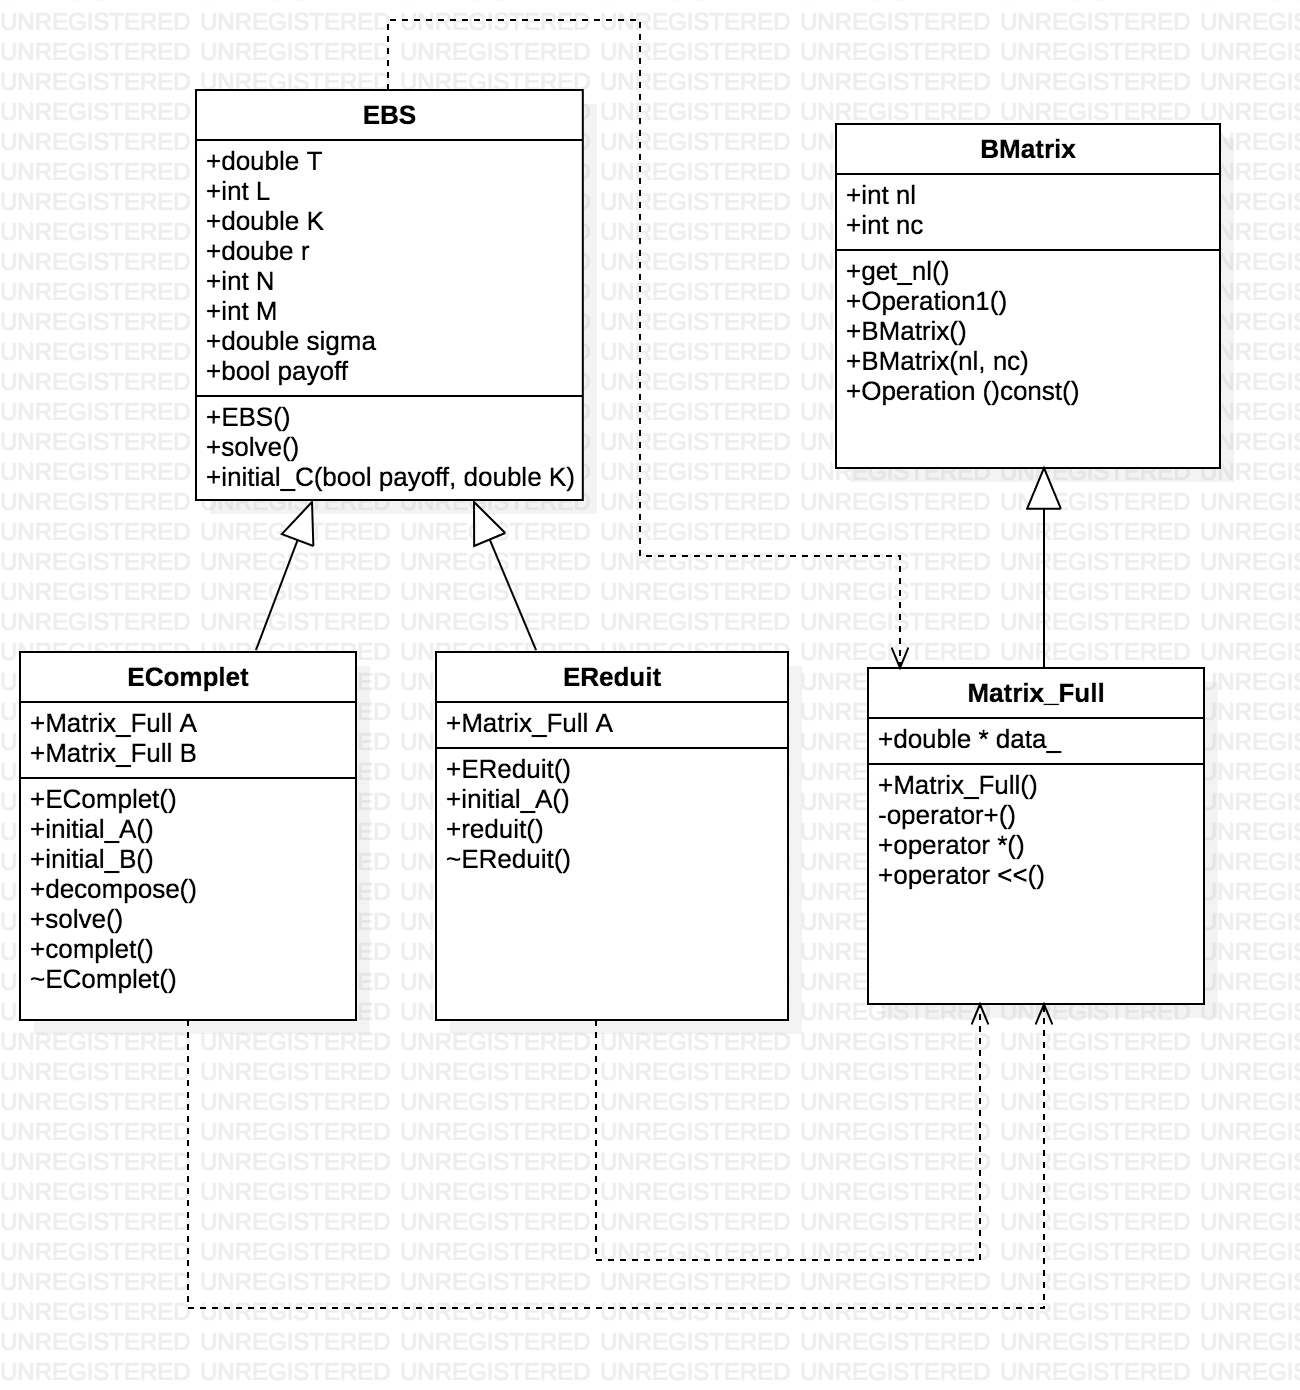
\includegraphics[scale=0.25]{Images/Main.png} 

Donc,  à partir d'initialiser la matrice A et B et C, on va parcourir chaque ligne de la matrice C
,on commence par Cn et on derminera quand qu'on trouvra la C0. Pour chaque itération on cherche à resoudre le problem $AC_i = BC_{i+1}$ ,on passe la matrice A à la méthode decompose et on appelle la méthode solve pour avoir la solution en donnant sa valeur à $C_i$ .

\section{Différence finie implicite}
\subsection{Transformer l'équation de Black-Scholes en une equation de chaleur}
NB : Pour simplifier les notations $\widetilde{S}$ sera vu comme $x$, $\widetilde{t}$ comme $\tau$ et $\widetilde{C}$ comme $u$.
Nous commençons par l'équation de Black-Scholes fournie dans le sujet :

$\frac{\partial C}{\partial t}+\frac{1}{2}\sigma^2S^2\frac{\partial^2 C}{\partial S^2}+ rS\frac{\partial C}{\partial S}=rC,\qquad\qquad\qquad\qquad\qquad(1)$

\subsubsection{Première étape}
L'équation peut être réecrite sous la forme équivalente :

$\frac{\partial C}{\partial t}+\frac{1}{2}\sigma^2\left(S\frac{\partial }{\partial S}\right)^2C+\left(r-\frac{1}{2}\sigma^2\right)S\frac{\partial C}{\partial S}-rC=0.$

Nous faisons un changement de variables :

$S=e^y,\qquad t=T-\tau$

Ce qui donne :

$S\frac{\partial }{\partial S}\to\frac{\partial}{\partial y},\qquad \frac{\partial}{\partial t}\to - \frac{\partial}{\partial \tau},$

Nous obtenons alors l'équation à coefficients constants suivante :

$\frac{\partial C}{\partial \tau}-\frac{1}{2}\sigma^2\frac{\partial^2 C}{\partial y^2}-\left(r-\frac{1}{2}\sigma^2\right)\frac{\partial C}{\partial y}+rC=0.\qquad\qquad\qquad(3)$

\subsubsection{Deuxième étape}
Si l'on remplace $C(y,\tau)$ dans l'équation (3) par  $u=e^{r\tau}C$, nous obtenons :

$\frac{\partial u}{\partial \tau}-\frac{1}{2}\sigma^2\frac{\partial^2 u}{\partial y^2}-\left(r-\frac{1}{2}\sigma^2\right)\frac{\partial u}{\partial y}=0.$

\subsubsection{Troisième étape}
Finalement, le changement de variable $x=y+(r-\sigma^2/2)\tau$ nous permet d'éliminer le terme de premier ordre et de mettre l'équation précédente sous la forme suivante :

$\frac{\partial u}{\partial \tau}=\frac{1}{2}\sigma^2\frac{\partial^2 u}{\partial x^2}$

\subsection{L'implémentation de la méthode des différences finies implicite}
\subsubsection{Documentation}
Considérons une équation de chaleur à une dimension vérifiée par $u$

$\frac{\partial u}{\partial t}=\alpha \frac{\partial^2 u}{\partial^2 x}$

Pour numériser l'équation précédente, il faut approximer les dérivées partielles par des différences. Dans ce cas l'on considère une grille spacio-temporelle $(x_i,t_i)$ homogène telle que la différence entre deux points de temps consécutifs soit $\Delta{t}$ et deux points de l'espace consécutifs soit $\Delta{x}$.

Les points $u(x_j,t_n)=u^n_j$ représenterons une approximation numérique de $u(x_j,t_n)$

Ainsi :

$\frac{\partial u}{\partial t}=\alpha \frac{\partial^2 u}{\partial^2 x}$

Est approximée en : 

$\frac{u^{n+1}_j-u^n_j}{\Delta{t}}=\alpha \frac{u^n_{j+1}-2u^n_j+u^n_{j-1}}{\Delta{x}^2}$

Ce qui donne : 

$u^{n+1}_j=\alpha \Delta{t} \frac{u^n_{j+1}-2u^n_j+u^n_{j-1}}{\Delta{x}^2}+u^n_j$

Nous posons $\beta = \frac{\alpha \Delta{t}}{\Delta{x}^2}$

L'équation précédente devient alors :

$u^{n+1}_j= \beta (u^n_{j+1}-2u^n_j+u^n_{j-1})+u^n_j$

Ce qui donne finalement : 

$u^{n+1}_j= \beta u^n_{j+1} +  (1-2\beta) u^n_j + \beta u^n_{j-1}$

Nous arrivons alors à une forme matricielle :

\[
A =
\left[ {\begin{array}{ccccccccc}

w & 0 & 0 & 0  & 0 & 0 & 0 & . & 0\\ 
a  & b  & c  & 0  & 0  & 0  & 0  & .  & 0 \\ 
0  & a  & b  & c  & 0  & 0  & 0  & .  & 0\\ 
.  & 0  & .  & .  & .  & 0  & 0  & 0  & 0\\ 
.  & 0  & 0  & .  & .  & .  & 0  & 0  & . \\
.  & 0  & 0  & 0  & .  & .  & .  & 0  & . \\
.  & 0  & 0  & 0  & 0  & .  & .  & .  & 0 \\
0  & .  & 0  & 0  & 0  & 0  & a  & b  & c\\ 
0  & .  & 0  & 0  & 0  & 0  & 0  & 0  & 1 \\
\end{array} } \right]
\]

ie une matrice dont tridiagonale en (a,b,c) à laquelle l'on rajoute une dernière ligne en (1,0,...,0) et une première ligne en ($w=\frac{u^{n+1}_0}{u^n_0}$,0,..,0)
à savoir $a=c=\beta$ et $b=1-2\beta$

Dans ce cas nous obtenons : 

$U^{n+1}=AU^n$
ie,
$U^n=A^{-1}U^{n+1}$

où
\[
U^{n+1} =
\left[ {\begin{array}{c}
        u^{n+1}_0\\
        .\\
        .\\
        .\\
        u^{n+1}_{M+1}\\
\end{array} } \right]
\]
        
Et évidemment 

\[
U^{n} =
\left[ {\begin{array}{c}
        u^{n}_0\\
        .\\
        .\\
        .\\
        u^{n}_{M+1}\\
\end{array} } \right]
\]
Commençant par la condition finale $U^T$, nous arrivons par boucle de T à 0 à $U^0$.




\newpage
\section{Affichage des courbes}

Le plot pour un put de la courbe avec la méthode complète :
\includegraphics[scale=0.25]{Images/Complet_put.png} 


Le plot pour un call de la courbe avec la méthode complète :
\includegraphics[scale=0.25]{Images/Complet_call.png} 


\end{document}
 
